% Name: Far commutativity
% Description: The relation σ₁σ₃ = σ₃σ₁: crossings on strands that are not neighbors can slide past each other.
% Tags: braid relation, braid group, commutativity

\usetikzlibrary{braids, calc}

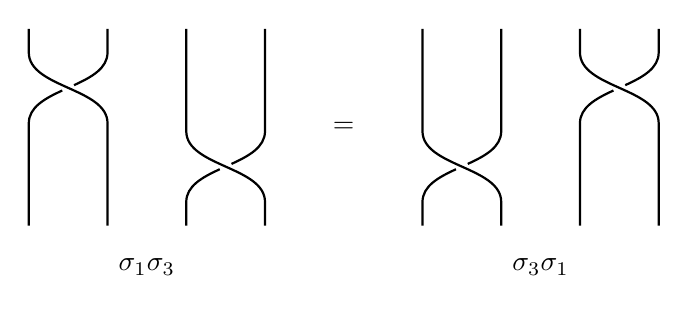
\begin{tikzpicture}
  \pic[braid/.cd, every strand/.style={thick}] (L) at (0,0) {braid={s_1 s_3}};
  \pic[braid/.cd, every strand/.style={thick}] (R) at (5,0) {braid={s_3 s_1}};
  \node at ($(L.east)!0.5!(R.west)$) {$=$};
  \node[below=3mm] at (L.south) {$\sigma_1\sigma_3$};
  \node[below=3mm] at (R.south) {$\sigma_3\sigma_1$};
\end{tikzpicture}
